\documentclass{sig-alternate}

\usepackage[utf8]{inputenc}
\usepackage[T1]{fontenc}
\usepackage[T1,T2A]{fontenc}
\usepackage{lmodern}
\usepackage[activate=compatibility]{microtype}

% autoref command
\usepackage[hyphens]{url}
\usepackage[pdftex,urlcolor=black,colorlinks=true,linkcolor=black,citecolor=black]{hyperref}
\def\sectionautorefname{Section}
\def\subsectionautorefname{Subsection}

\usepackage{enumitem}

\usepackage{color}
\definecolor{light-gray}{gray}{0.8}

% todo macro
\usepackage{color}
\newcommand{\todo}[1]{\noindent\textcolor{red}{{\bf \{TODO}: #1{\bf \}}}}

% nicer looking Google+
\usepackage{xspace}
\DeclareRobustCommand{\googleplus}{\mbox{Google\hspace{0em}\raisebox{.28ex}{\tiny\bf +}\kern-0.2ex}\xspace}

% listings and Verbatim environment
\usepackage{fancyvrb}
\usepackage{relsize}
\usepackage{listings}
\usepackage{verbatim}
\newcommand{\defaultlistingsize}{\fontsize{8pt}{9.5pt}}
\newcommand{\inlinelistingsize}{\fontsize{8pt}{11pt}}
\newcommand{\smalllistingsize}{\fontsize{7.5pt}{9.5pt}}
\newcommand{\listingsize}{\defaultlistingsize}
\RecustomVerbatimCommand{\Verb}{Verb}{fontsize=\inlinelistingsize}
\RecustomVerbatimEnvironment{Verbatim}{Verbatim}{fontsize=\defaultlistingsize}
\lstset{frame=lines,captionpos=b,numberbychapter=false,escapechar=§,
        aboveskip=2em,belowskip=1em,abovecaptionskip=0.5em,belowcaptionskip=0.5em,
        framexbottommargin=-1em,basicstyle=\ttfamily\listingsize\selectfont}

% use Courier from this point onward
\let\oldttdefault\ttdefault
\renewcommand{\ttdefault}{pcr}
\let\oldurl\url
\renewcommand{\url}[1]{\inlinelistingsize\oldurl{#1}}

\lstdefinelanguage{JavaScript}{
  keywords={push, typeof, new, true, false, catch, function, return, null, catch, switch, var, if, in, while, do, else, case, break},
  keywordstyle=\bfseries,
  ndkeywords={class, export, boolean, throw, implements, import, this},
  ndkeywordstyle=\color{darkgray}\bfseries,
  identifierstyle=\color{black},
  sensitive=false,
  comment=[l]{//},
  morecomment=[s]{/*}{*/},
  commentstyle=\color{darkgray},
  stringstyle=\color{red},
  morestring=[b]',
  morestring=[b]"
}

% linewrap symbol
\definecolor{grey}{RGB}{130,130,130}
\newcommand{\linewrap}{\raisebox{-.6ex}{\textcolor{grey}{$\hookleftarrow$}}}

\hyphenation{Wikistream Wikipedia Wikipedias}

%\def\baselinestretch{0.99}

\begin{document}

% --- Author Metadata here ---
\conferenceinfo{World Wide Web Conference}{'13 Rio de Janeiro, Brazil}
\CopyrightYear{2013} % Allows default copyright year (20XX) to be over-ridden - IF NEED BE.
%\crdata{0-12345-67-8/90/01}  % Allows default copyright data (0-89791-88-6/97/05) to be over-ridden - IF NEED BE.
% --- End of Author Metadata ---


\title{A Meteoroid on Steroids: Ranking Media Items\\ Stemming from Social Networks}

\numberofauthors{1}\author{
\alignauthor
Thomas Steiner\\
	\affaddr{Google Germany GmbH}\\
	\affaddr{ABC-Str. 19}\\
	\affaddr{20354 Hamburg, Germany}\\
	\email{tomac@google.com} 
}
\maketitle

\begin{abstract}
We have developed an application called Social Media Illustrator
that allows for searching for media items on multiple social networks,
clustering them by visual similarity, ranking them by different criteria,
and finally arranging them in aesthetically attractive media galleries.
In this paper, we focus on the ranking aspect and show how 
The application is available publicly online at \url{http://social-media-illustrator.herokuapp.com/}.
\end{abstract}

\category{H.3.3}{Information Search and Retrieval}{Clustering}

\terms{Algorithms}

\keywords{}

\section{Introduction}

\begin{figure*}[t!]
  \centering
  \fcolorbox{light-gray}{white}{
  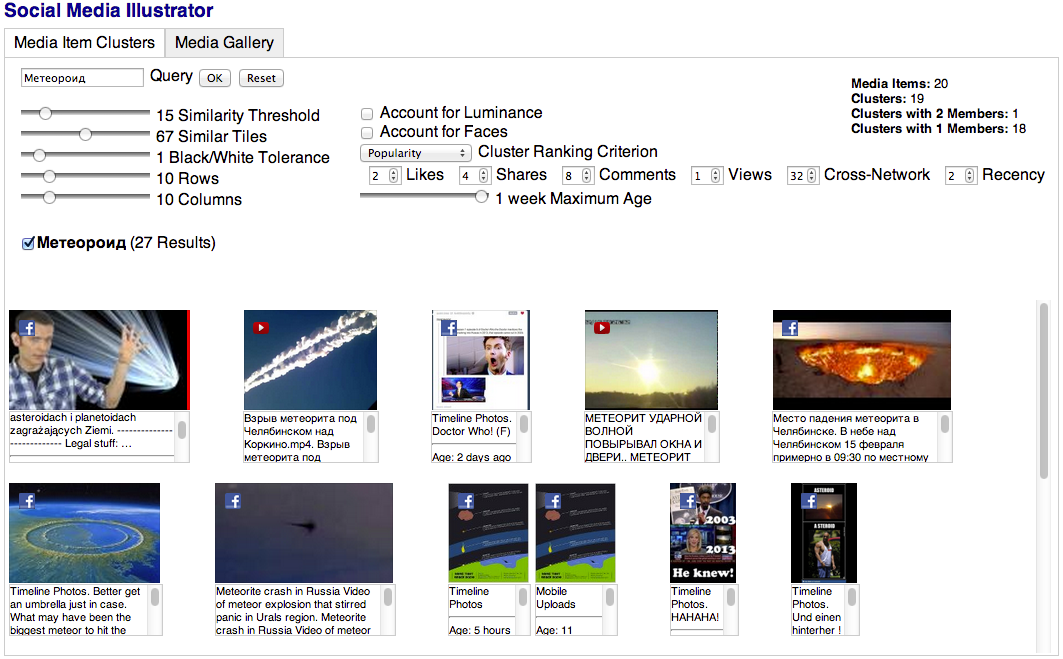
\includegraphics[width=\linewidth]{./application.png}}
  \caption{Media item clusters tab of the Social Media Illustrator application
  with individual and clustered (bottom middle) media items from Facebook and YouTube,
  ranked by popularity for the Russian query
    \fontencoding{T2A}\selectfont Метеороид \fontencoding{T1}\selectfont}
  \label{fig:application}
\end{figure*}

\begin{figure*}[t!]
  \centering
  \fcolorbox{light-gray}{white}{
  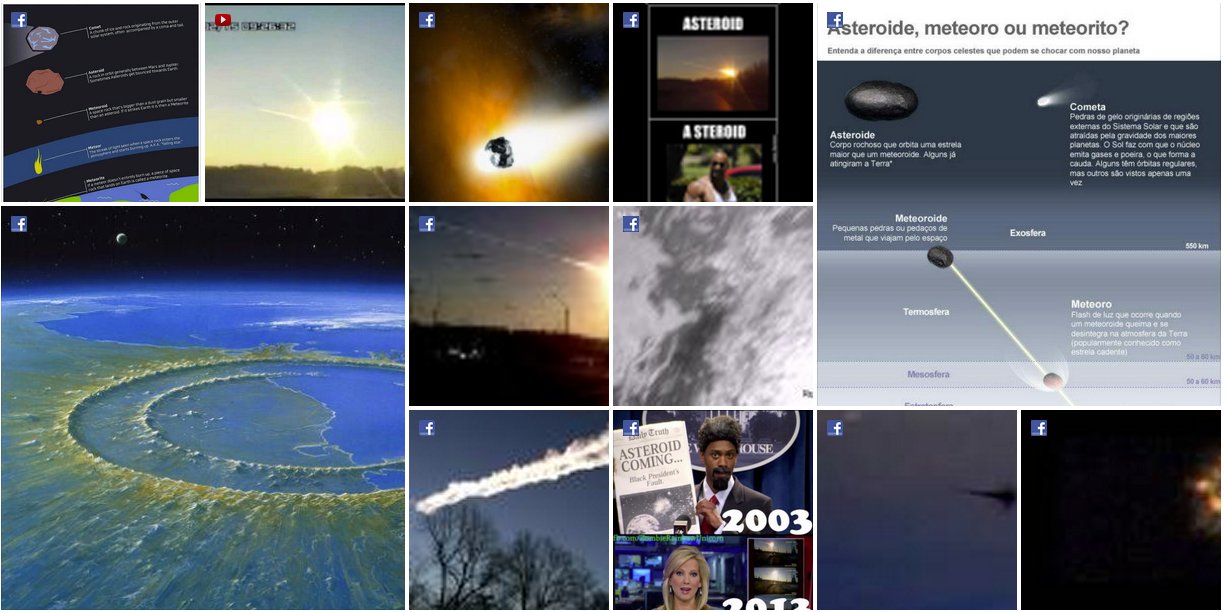
\includegraphics[width=\linewidth]{./media-gallery.png}}
  \caption{Automatically generated media gallery in \emph{loose order, varying size} style
    showcasing ranked media items stemming from Facebook and YouTube for the Russian query
    \fontencoding{T2A}\selectfont Метеороид \fontencoding{T1}\selectfont}
  \label{fig:media-gallery}
\end{figure*}

\bibliographystyle{abbrv}
\bibliography{www2013devtrack}

\end{document}